\section{Общие сведения теории формальных языков}

В данной главе мы рассмотрим основные понятия из теории формальных языков, которые пригодятся нам в дальнейшем изложении.

\begin{definition}
\textit{Алфавит} --- это конечное множество.
Элементы этого множества будем называть \textit{символами}.
\end{definition}

\begin{example}
  Примеры алфавитов

  \begin{itemize}
    \item Латинский алфавит $\Sigma = \{ a, b, c, \dots, z\}$
    \item Кириллический алфавит $\Sigma = \{ \text{а, б, в, \dots, я}\}$
    \item Алфавит чисел в шестнадцатеричной записи $\Sigma = \{0, 1, 2, 3, 4, 5, 6, 7 ,8,9, A, B, C, D, E, F \}$
  \end{itemize}
\end{example}

Традиционное обозначение для алфавита --- $\Sigma$.
Также мы будем использовать различные прописные буквы латинского алфавита. Для обозначения символов алфавита будем использовать строчные буквы латинского алфавита: $a, b, \dots, x, y, z$.

Будем считать, что над алфавитом $\Sigma$ всегда определена операция конкатенации $(\cdot): \Sigma^* \times \Sigma^* \to \Sigma^*$.
При записи выражений символ точки (обозначение операции конкатенации) часто будем опускать: $a \cdot b = ab$.

\begin{definition}
\textit{Слово} над алфавитом $\Sigma$ --- это конечная конкатенация символов алфавита $\Sigma$: $\omega = a_0 \cdot a_1 \cdot \ldots \cdot a_m$, где $\omega$ --- слово, а для любого $i$ $a_i \in \Sigma$.
\end{definition}

\begin{definition}
\textit{Слово} над алфавитом $\Sigma$ --- это результат конечной конкатенации символов алфавита $\Sigma$: $\omega = a_0 \cdot a_1 \cdot \ldots \cdot a_m$, где $\omega$ --- слово, а для любого $i$ $a_i \in \Sigma$.
Будем называть $m + 1$ длиной слова и обозначать как $|\omega|$.
\end{definition}

\begin{definition}
\textit{Язык} над алфавитом $\Sigma$ --- это множество слов над алфавитом $\Sigma$.
\end{definition}

\begin{example}
  Примеры языков

  \begin{itemize}
    \item Язык целых чисел в двоичной записи $\{0, 1, -1, 10, 11, -10, -11, \dots\}$
    \item Язык всех правильных скобочных последовательностей $\{(), (()), ()(), (())(), \dots\}$
  \end{itemize}
\end{example}

Любой язык над алфавитом $\Sigma$ является подмножеством $\Sigma^*$ --- множества всех слов над алфавитом $\Sigma$

Заметим, что язык не обязан быть конечным множеством, в то время как алфавит всегда конечен и изучаем мы конечные слова.

%\begin{definition}
\textit{Способы задания языков}
\begin{itemize}
\item Перечислить все элементы. Такой способ работает только для конечных языков. Перечислить бесконечное множество не получится.
\item Задать генератор --- процедуру, которая возвращает очередное слово языка.
\item Задаьть распознователь --- процедуру, которая по данному слову может определить, принадлежит оно заданному языку ли нет.
\end{itemize}


\subsection{Контекстно-свободные грамматики и языки}

Из всего многообразия нас будут интересовать прежде всего контекстно-свободные грамматики.

\begin{definition}
\textit{Контекстно-свободная грамматика} --- это четвёрка вида $\langle \Sigma, N, P, S \rangle$, где
\begin{itemize}
  \item $\Sigma$ --- это терминальный алфавит;
  \item $N$ --- это нетерминальный алфавит;
  \item $P$ --- это множество правил или продукций, таких что каждая продукция имеет вид $N_i \to \alpha$, где $N_i \in N$ и $\alpha \in \{\Sigma \cup N\}^* \cup {\varepsilon}$;
  \item $S$ --- стартовый нетерминал.
  Отметим, что $\Sigma \cap N = \varnothing$.
\end{itemize}
\end{definition}

\begin{example}
Грамматика, задающая язык целых чисел в двоичной записи без лидирующих нулей: $G = \langle \{0, 1, -\}, \{S, N, A\}, P, S \rangle$, где $P$ определено следующим образом:

\[
\begin{array}{rcl}
S& \rightarrow & 0 \mid N \mid - N  \\
N& \rightarrow & 1 A \\
A& \rightarrow & 0 A \mid 1 A  \mid \varepsilon\\
\end{array}
\]
\end{example}

При спецификации грамматики часто опускают множество терминалов и нетерминалов, оставляя только множество правил. При этом нетерминалы часто обозначаются прописными латинскими буквами, терминалы --- строчными, а стартовый нетерминал обозначается буквой~$S$. Мы будем следовать этим обозначениям, если не указано иное.


\begin{definition}
  \textit{Отношение непосредственной выводимости}. Мы говорим, что последовательность терминалов и нетерминалов $\gamma \alpha \delta$ \textit{непосредственно выводится из} $\gamma \beta \delta$ \textit{при помощи правила} $\alpha \rightarrow \beta$ ($\gamma \alpha \delta \Rightarrow \gamma \beta \delta$), если
  \begin{itemize}
    \item $\alpha \rightarrow \beta \in P$
    \item $\gamma, \delta \in \{\Sigma \cup N\}^* \cup {\varepsilon}$
  \end{itemize}
\end{definition}

\begin{definition}
\textit{Отношение выводимости} является рефлексивно-транзитивным замыканием отношения непосредственной выводимости
\begin{itemize}
  \item $\alpha \derives \beta$ означает $\exists \gamma_0, \dots \gamma_k: \ \alpha \derives[] \gamma_0 \derives[] \gamma_1 \derives[] \dots \derives[] \gamma_{k-1} \derives[] \gamma_{k} \derives[] \beta$
  \item Транзитивность: $\forall \alpha, \beta, \gamma \in \{\Sigma \cup N\}^* \cup {\varepsilon}: \ \alpha \derives \beta, \beta \derives \gamma \Rightarrow \alpha \derives \gamma$
  \item Рефлексивность: $\forall \alpha \in \{\Sigma \cup N\}^* \cup {\varepsilon}: \ \alpha \derives \alpha$
  \item $\alpha \derives \beta$ --- $\alpha$ выводится из $\beta$
  \item $\alpha \derives[k] \beta$ --- $\alpha$ выводится из $\beta$ за $k$ шагов
  \item $\alpha \derives[+] \beta$ --- при выводе использовалось хотя бы одно правило грамматики
\end{itemize}
\end{definition}


\begin{example}
Пример вывода цепочки $-1101$ в грамматике:

  \[
  \begin{array}{rcl}
  S& \rightarrow & 0 \mid N \mid - N  \\
  N& \rightarrow & 1 A \\
  A& \rightarrow & 0 A \mid 1 A  \mid \varepsilon\\
  \end{array}
  \]

  \[ S \Rightarrow - N \Rightarrow - 1 A \Rightarrow - 1 1 A \derives - 1 1 0 1 A \Rightarrow - 1 1 0 1 \]
\end{example}






\begin{definition}
  \textit{Рефлексивно-транзитивное замыкание отношения} --- это наименьшее рефлексивное и транзитивное отношение, содержащее исходное.
  \end{definition}

\begin{definition}
\textit{Вывод слова в грамматике}. Слово $\omega \in \Sigma^*$ \textit{выводимо в грамматике} $\langle \Sigma, N, P, S \rangle$, если существует некоторый вывод этого слова из начального нетерминала $S \derives \omega$.

\end{definition}

\begin{definition}
\textit{Левосторонний вывод}. На каждом шаге вывода заменяется самый левый нетерминал.
\end{definition}

\begin{example}
Пример левостороннего вывода цепочки в грамматике

  \[
    \begin{array}{rcl}
    S& \rightarrow & A A \mid s  \\
    A& \rightarrow & A A \mid B b \mid a \\
    B& \rightarrow & c \mid d
    \end{array}
  \]

  \[ \boldsymbol{S} \derives[] \boldsymbol{A} A \derives[] \boldsymbol{B} b A \derives[] c b \boldsymbol{A} \derives[] c b \boldsymbol{A} A \derives[] c b a \boldsymbol{A} \derives[] c b a a \]
\end{example}

Аналогично можно определить правосторонний вывод.

\begin{definition}
\textit{Язык, задаваемый грамматикой} --- множество строк, выводимых в грамматике $L(G) = \{ \omega \in \Sigma^* \mid S \derives \omega \}$.
\end{definition}

\begin{definition}
  Грамматики $G_1$ и $G_2$ называются \textit{эквивалентными}, если они задают один и тот же язык: $L(G_1) = L(G_2)$
\end{definition}


\begin{example}  Пример эквивалентных грамматик для языка целых чисел в двоичной системе счисления.

  \begin{tabular}{p{0.4\textwidth} | p{0.5\textwidth}}

    \[
      \begin{array}{rcl}
      \Sigma &=& \{ 0, 1, - \} \\
      N &=& \{ S, N, A \} \\~\\
      S& \rightarrow & 0 \mid N \mid - N  \\
      N& \rightarrow & 1 A \\
      A& \rightarrow & 0 A \mid 1 A  \mid \varepsilon\\
      \end{array}
    \]

    &

    \[
      \begin{array}{rcl}
      \Sigma &=& \{ 0, 1, - \} \\
      N &=& \{ S, A \} \\~\\
      S& \rightarrow & 0 \mid 1 A  \mid - 1 A  \\
      A& \rightarrow &  0 A \mid 1 A  \mid \varepsilon\\
      \end{array}
    \]
    \end{tabular}

\end{example}


\begin{definition}
  \textit{Неоднозначная грамматика} --- грамматика, в которой существует 2 и более выводов для одного слова.
\end{definition}

\begin{example}
  Неоднозначная грамматика для правильных скобочных последовательностей

\[
    S \to (S) \mid S S \mid \varepsilon
\]
\end{example}

\begin{definition}
  \textit{Однозначная грамматика} --- грамматика, в которой существует не более одного вывода для каждого слова.
\end{definition}

\begin{example}
  Однозначная грамматика для правильных скобочных последовательностей

\[
    S \to (S)S \mid \varepsilon
\]
\end{example}

\begin{definition}
  \textit{Существенно неоднозначные языки} --- язык, для которого невозможно построить однозначную грамматику
\end{definition}

\begin{example}
  Пример существенно неоднозначного языка

\[\{a^n b^n c^m \mid n, m \in \mathds{Z}\} \cup \{a^n b^m c^m \mid n,m \in \mathds{Z}\}\]
\end{example}

\subsection{Дерево вывода}\label{sect:DerivTree}
В некоторых случаях не достаточно знать порядок применения правил.
Необходимо структурное представление вывода цепочки в грамматике.
Таким представлением является \textit{дерево вывода}.
\begin{definition}
Деревом вывода цепочки $\omega$ в грамматике $G=\langle \Sigma, N, S, P \rangle$ называется дерево, удовлетворяющее следующим свойствам.

\begin{enumerate}
  \item Помеченное: метка каждого внутреннего узла --- нетерминал, метка каждого листа --- терминал или $\varepsilon$.
  \item Корневое: корень помечен стартовым нетерминалом.
  \item Упорядоченное.
  \item В дереве есть узел с меткой $N_i$ и сыновьями $M_j \dots M_k$ тогда и только тогда, когда в грамматике есть правило вида $N_i \to M_j \dots M_k$.
  \item Крона образует цепочку.
\end{enumerate}
\end{definition}

\begin{example}
  Построим дерево вывода цепочки $ababab$ в грамматике

  \[ G = \langle \{a,b\}, \{S\}, S, \{S \to a \ S \ b \ S, S \to \varepsilon\} \rangle \]

\begin{center}

    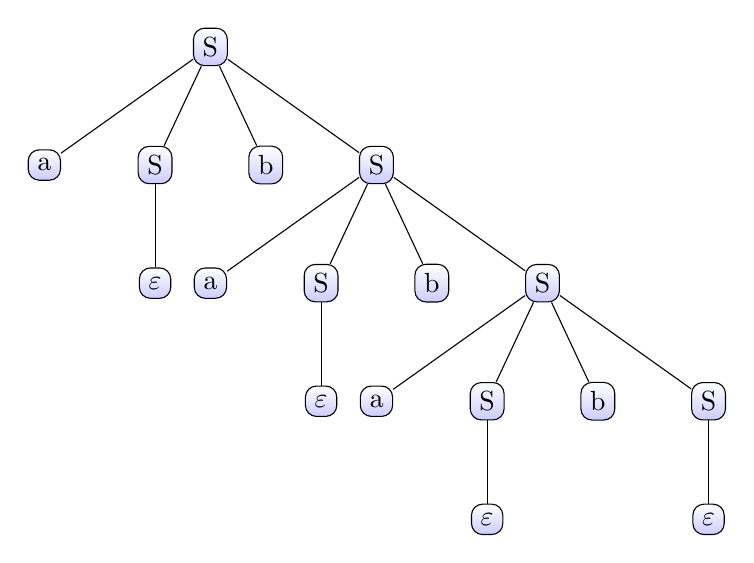
\begin{tikzpicture}[sibling distance=4em,
    every node/.style = {shape=rectangle, rounded corners,
      draw, align=center,
      top color=white, bottom color=blue!20}]]
    \node {S}
      child { node {a} }
      child { node {S}
        child { node {$\varepsilon$}}
      }
      child { node {b} }
      child { node {S}
        child {node {a}}
        child { node {S}
          child { node {$\varepsilon$}}
        }
        child { node {b} }
        child { node {S}
          child {node {a}}
          child {node {S}
            child {node {$\varepsilon$}}
          }
          child {node {b}}
          child {node {S}
            child {node {$\varepsilon$}}
          }
        }
      };
  \end{tikzpicture}
\end{center}

\end{example}

\begin{theorem}
  Пусть $G = \langle \Sigma, N, P, S \rangle$ --- КС-грамматика.
  Вывод $S \derives \alpha$, где $\alpha \in (N \cup \Sigma)^*, \alpha \neq \varepsilon$ существует $\Leftrightarrow$ существует дерево вывода в грамматике $G$ с кроной $\alpha$.
\end{theorem}

\subsection{Пустота КС-языка}

\begin{theorem}
  Существует алгоритм, определяющий, является ли язык, порождаемый КС грамматикой, пустым
\end{theorem}

\begin{proof}
  Следующая лемма утверждает, что если в КС языке есть выводимое слово, то существует другое выводимое слово с деревом вывода не глубже количества нетерминалов грамматики.
  Для доказательства теоремы достаточно привести алгоритм, последовательно строящий все деревья глубины не больше количества нетерминалов грамматики, и проверяющий, являются ли такие деревья деревьями вывода.
  Если в результате работы алгоритма не удалось построить ни одного дерева, то грамматика порождает пустой язык.
\end{proof}

\begin{lemma}
  Если в данной грамматике выводится некоторая цепочка, то существует цепочка, дерево вывода которой не содержит ветвей длиннее m, где m --- количество нетерминалов грамматики
\end{lemma}

\begin{proof}
  Рассмотрим дерево вывода цепочки $\omega$. Если в нем есть 2 узла, соответствующих одному нетерминалу A, обозначим их $n_1$ и $n_2$.

  Предположим, $n_1$ расположен ближе к корню дерева, чем $n_2$.

  $S \derives \alpha A_{n_1} \beta \derives \alpha \omega_1 \beta; S \derives \alpha \gamma A_{n_2} \delta \beta \derives \alpha \gamma \omega_2 \delta \beta$, при этом $\omega_2$ является подцепочкой $\omega_1$.

  Заменим в изначальном дереве узел $n_1$ на $n_2$. Полученное дерево является деревом вывода $\alpha \omega_2 \delta$.

  Повторяем процесс замены одинаковых нетерминалов до тех пор, пока в дереве не останутся только уникальные нетерминалы.

  В полученном дереве не может быть ветвей длины большей, чем m.

  По построению оно является деревом вывода.
\end{proof}


\subsection{Нормальная форма Хомского}
\label{section:CNF}

\begin{definition}
Контекстно-свободная грамматика $\langle \Sigma, N, P, S\rangle$ находится в \textit{Нормальной Форме Хомского}, если она содержит только правила следующего вида:

\begin{itemize}
  \item $A \to B C \text{, где } A, B, C \in N^* $
  \item $A \to a \text{, где } A \in N, a \in \Sigma$
  \item $S \to \varepsilon$
\end{itemize}
\end{definition}

\begin{theorem}
Любую КС грамматику можно преобразовать в НФХ.
\end{theorem}

\begin{proof}
  Алгоритм преобразования в НФХ состоит из следующих шагов:

  \begin{itemize}
    \item Замена неодиночных терминалов
    \item Удаление длинных правил
    \item Удаление $\varepsilon$-правил
    \item Удаление цепных правил
    \item Удаление бесполезных нетерминалов
  \end{itemize}

  То, что каждый из этих шагов преобразует грамматику к эквивалентной, при этом является алгоритмом, доказано в следующих леммах.
\end{proof}

\begin{lemma}
  Для любой КС-грамматики можно построить эквивалентную, которая не содержит правила с неодиночными терминалами.
\end{lemma}

\begin{proof}
  Каждое правило $A \to B_0 B_1 \dots B_k, k \geq 1$ заменить на множество правил:
  \begin{itemize}
    \item $A \to C_0 C_1 \dots C_k$
    \item $\{ C_i \to B_i \mid B_i \in \Sigma, C_i \text{ --- новый нетерминал} \}$
  \end{itemize}
\end{proof}

\begin{lemma}
  Для любой КС-грамматики можно построить эквивалентную, которая не содержит правил длины больше 2.
\end{lemma}

\begin{proof}
  Каждое правило $A \to B_0 B_1 \dots B_k, k \geq 2$ заменить на множество правил:
  \begin{itemize}
    \item $A \to B_0 C_0$
    \item $C_0 \to B_1 C_1$
    \item $\dots$
    \item $C_{k-3} \to B_{k-2} C_{k-2}$
    \item $C_{k-2} \to B_{k-1} B_k$
  \end{itemize}
\end{proof}


\begin{lemma}
  Для любой КС-грамматики можно построить эквивалентную, не содержащую $\varepsilon$-правил.
\end{lemma}

\begin{proof}
  Определим $\varepsilon$-правила:
  \begin{itemize}
    \item $A \to \varepsilon$
    \item $A \to B_0 \dots B_k, \forall i: \ B_i$ --- $\varepsilon$-правило.
  \end{itemize}

  Каждое правило $A \to B_0 B_1 \dots B_k$ заменяем на множество правил, где каждое $\varepsilon$-правило удалено во всех возможных комбинациях.
\end{proof}

\begin{lemma}
  Можно удалить все цепные правила
\end{lemma}

\begin{lemma}
  Можно удалить все бесполезные нетерминалы
\end{lemma}

\begin{example}
  Приведем в Нормальную Форму Хомского однозначную грамматику правильных скобочных последовательностей: $S \to a S b S \mid \varepsilon$

  Первым шагом добавим новый нетерминал и сделаем его стартовым: 

  \begin{align*}
    S_0 &\to S  \\ 
    S   &\to a S b S \mid \varepsilon
  \end{align*}

  Заменим все терминалы на новые нетерминалы: 

  \begin{align*}
    S_0 &\to S \\ 
    S   &\to L S R S \mid \varepsilon \\ 
    L   &\to a \\ 
    R   &\to b
  \end{align*}

  Избавимся от длинных правил: 

  \begin{align*}
    S_0 &\to S \\ 
    S   &\to L S' \mid \varepsilon \\ 
    S'  &\to S S'' \\ 
    S'' &\to R S \\
    L   &\to a \\ 
    R   &\to b
  \end{align*}

  Избавимся от $\varepsilon$-продукций: 

  \begin{align*}
    S_0 &\to S \mid \varepsilon \\ 
    S   &\to L S' \\ 
    S'  &\to S'' \mid S S'' \\ 
    S'' &\to R   \mid R S \\
    L   &\to a \\ 
    R   &\to b
  \end{align*}

  Избавимся от цепных правил: 

  \begin{align*}
    S_0 &\to L S' \mid \varepsilon \\ 
    S   &\to L S' \\ 
    S'  &\to b \mid R S \mid S S'' \\ 
    S'' &\to b \mid R S \\
    L   &\to a \\ 
    R   &\to b
  \end{align*}
\end{example}

\subsection{Вопросы и задачи}
\begin{enumerate}
  \item Предъявить несколько выводов для одной цепочки.
  \item Построить выводы
  \item Построить деревья вывода !!! Перенести из раздела про SPPF
\end{enumerate}
